\section{Kompilierung und Programmierung}\label{section:prototypische-implementierung:kompilierung-und-programmierung}

Für die Kompilierung wurde in der prototypischen Implementierung das \ac{Arduino CLI} \cite{noauthor_arduino-cli_nodate} verwendet. Dieses nutzt intern den Compiler \ac{GCC} \cite{noauthor_gcc_nodate}. Neben der Kompilierung des Quellcodes werden auch Arduino spezifische Vorverarbeitungsschritte durchgeführt. Dadurch können Nutzer auch ggf. ihnen bereits bekannte Arduino Funktionen wie z.B. \texttt{digitalWrite()} und \texttt{digitalRead()} nutzen. Im Allgemeinen sollte dadurch die Programmierung der Microcontroller für die Nutzer vereinfacht werden. Um das \ac{Arduino CLI} zur Kompilierung innerhalb eines Experiments nutzen zu können, muss dieses als ein entsprechendes Laborgerät bereitgestellt werden. Dafür wurde ein cloud-instanziierbares Laborgerät entwickelt. Dieses bietet einen entsprechenden Compilation Service Producer an, welcher während einem Experiment mit der IDE verbunden werden kann. Das instanziierte Laborgerät nimmt die entsprechenden Kompilieranfragen entgegen und bearbeitet diese. Sollte die Kompilierung erfolgreich sein, wird eine entsprechende Antwort mit dem Ergebnis der Kompilierung an die IDE gesendet. Im Fehlerfall wird die Fehlermeldung des Compilers in der Antwort mitgesendet.

\begin{figure}[tbp]
    \centering
    \begin{tikzpicture}
        \begin{class}[text width=6.5cm]{CompilationServiceProducer}{0,0}
            \operation{+ addResultFormat()}
            \operation{+ onCompile()}
        \end{class}
        \begin{class}[text width=6.5cm]{CompilationServiceConsumer}{7.5,0}
            \operation{+ compile()}
        \end{class}
        \begin{class}[text width=6.5cm]{ProgrammingServiceProducer}{0,-2.5}
            \operation{+ onProgram()}
        \end{class}
        \begin{class}[text width=6.5cm]{ProgrammingServiceConsumer}{7.5,-2.5}
            \operation{+ program()}
        \end{class}
    \end{tikzpicture}
    \caption{Klassendiagramm Compilation Service \& Programming Service}
    \label{figure:klassendiagramm-compilation-service}
\end{figure}

In \autoref{figure:klassendiagramm-compilation-service} ist ein Klassendiagramm für den Compilation Service und den Programming Service gegeben. Hierbei besitzt der Compilation Service Consumer nur die Funktion \texttt{compile()}, welche verwendet werden kann um eine Kompilieranfrage an den Compilation Service Producer zu senden. Dieser löst ein \texttt{Compile}-Event aus, das über entsprechende Event-Handler behandelt werden kann. Zusätzlich besitzt der Compilation Service Producer noch die Funktion \texttt{addResultFormat()} um mögliche Ausgabeformate der Kompilierung zu registrieren. Der Programming Service Producer besitzt nur die Funktion \texttt{program()}, welche verwendet werden kann um eine Programmieranfrage an den Programming Service Producer zu senden. Dieser löst ein \texttt{Program}-Event aus, das über entsprechende Event-Handler behandelt werden kann.

\begin{figure}[tbp]
    \centering
    \begin{tikzpicture}
        \node[anchor=south west,inner sep=0] at (0,0) {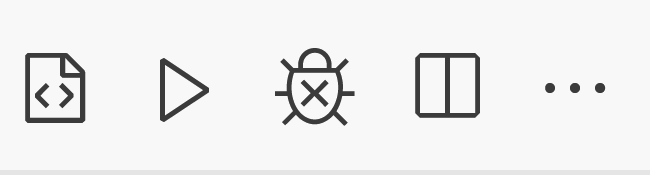
\includegraphics[trim={0 0 14.6cm 0},clip,width=0.2\textwidth]{images/symbols.png}};
        \draw[orange,ultra thick,rounded corners] (0.1,0.4) rectangle (1.4,1.85);
        \draw[blue!60,ultra thick,rounded corners] (1.8,0.4) rectangle (3.0,1.85);
        \node[orange] at (-1.5,1) {Kompilierung};
        \node[blue!60] at (4.9,1) {Programmierung};
    \end{tikzpicture}
    \caption{Schaltflächen für die Kompilierung \& Programmierung}
    \label{figure:benutzerinterface:symbole}
\end{figure}

Um die Kompilierung und die Programmierung von Steuereinheiten über der IDE ausführen zu können, wurde eine entsprechende Erweiterung entwickelt. Diese wird im Folgenden als \textit{Compilation Erweiterung} bezeichnet und fügt neben einem Compilation Service Consumer sowie einem Programming Service Consumer auch zwei Bedienelemente hinzu. Dabei werden eine Schaltfläche zur Kompilierung des aktuellen Projekts sowie eine weitere Schaltfläche zur Kompilierung und anschließenden Programmierung der Steuereinheit bereitgestellt. Diese werden in \autoref{figure:benutzerinterface:symbole} gezeigt. Die erste Schaltfläche kann dazu genutzt werden, um zu überprüfen, ob das aktuelle Projekt kompiliert werden kann und um die entsprechenden Mitteilungen vom Compiler zu erhalten. Die zweite Schaltfläche führt auch eine Kompilierung des aktuellen Projekts durch und zeigt entsprechende Rückmeldungen an. Sollte die Kompilierung erfolgreich sein, wird anschließend das Ergebnis dieser über den Programming Service Consumer an die zu programmierende Steuereinheit gesendet. In einer kollaborativen Sitzung ist das Kompilieren von Projekten stets erlaubt. Allerdings wird das Hochladen von Projekten deaktiviert, falls ein anderer Nutzer aktuell ein Projekt auf die Steuereinheit hochlädt oder falls die Steuereinheit in einer Debug-Sitzung verwendet wird.

Die betrachtete Experimentkonfiguration wird um das erstellte Laborgerät für die Bereitstellung des Arduino CLI erweitert. Dieses wird über den Compilation Service mit den IDEs verbunden. Zusätzlich wird die Steuereinheit um einen Programming Service Producer erweitert. Dadurch können die IDEs über den Programming Service mit der Steuereinheit verbunden werden (sh. \autoref{figure:experimentkonfiguration:kompilierung}).